% -----------------------------------------------------------------------------
%   Arquivo: ./01-texto/desenvolvimento.tex
% -----------------------------------------------------------------------------


\section{Desenvolvimento}\label{sec:desenvolvimento}	% edite para alterar o título da seção


Caso seja conveniente, podem ser criadas outras seções para o desenvolvimento do artigo. No entanto, as seções de introdução e conclusão são obrigatórias.

Para desmembrar esta seção em quantas forem necessárias/convenientes, copie este arquivo, renomeie-o e lembre-se de editar o arquivo "meuArtigo.tex" para incluir os arquivos criados para cada nova seção.

Organize o seu artigo científico da maneira mais conveniente para o leitor do trabalho. É para ele que você escreve.

Normalmente, esta seção "Desenvolvimento" não é utilizada na prática. Pode ser mais adequado substituí-la por três seções: "Fundamentação teórica", "Experimentos", "Análise e discussão dos resultados", ou outra organização de texto que o autor julgue mais vantajosa.

Qualquer que seja a organização escolhida, o que não pode faltar de forma alguma no corpo do texto descritivo de seu trabalho de pesquisa é o "quê" você fez de fato, em detalhes suficientes para que um outro pesquisador possa compreender.

Também não pode faltar a metodologia, ou seja, "como" você fez o trabalho, bem detalhado para que outros possam reproduzir seus experimentos ou ensaios ou seja lá o que foi feito e que possa obter os mesmos resultados que você obteve. Isso significa que todas as condições iniciais e de contorno, bem como todos os valores de variáveis devem estar indicados no texto. Faz parte da metodologia de pesquisa apresentar e discutir como os dados são analisados, se fez um tratamento estatístico neles ou não, e porquê. Finalmente, você deve apresentar seus resultados de maneira clara e objetiva, usando e abusando de gráficos e tabelas para facilitar a compreensão do leitor.

Uma questão que sempre surge é se é mais adequado apresentar "todos" os resultados primeiro e "depois" discute-los, ou se seria mais conveniente organizar os resultados em "blocos" que seriam apresentados e discutidos  bloco a bloco. A resposta é: isto fica a critério do autor do trabalho. O essencial é que fique compreensível ara o leitor do trabalho.

$x(t)=0.01681*e^{0.932x} + 1.532*10^{-16}*e^{3.653x}, \textrm{ }x=\textrm{tamanho entrada}$



% -----------------------------------------------------------------------------
% Nova subseção
% -----------------------------------------------------------------------------

\subsection{Figura ocupando uma coluna}		% edite para alterar o título da subseção

A \textbf{Figura \ref{fig:patoA}} foi inserida, em uma única coluna, utilizando os comandos abaixo.

\begin{center}
  \captionof{figure}{Pato na lagoa. Fator de escala: 8\% da original} 
  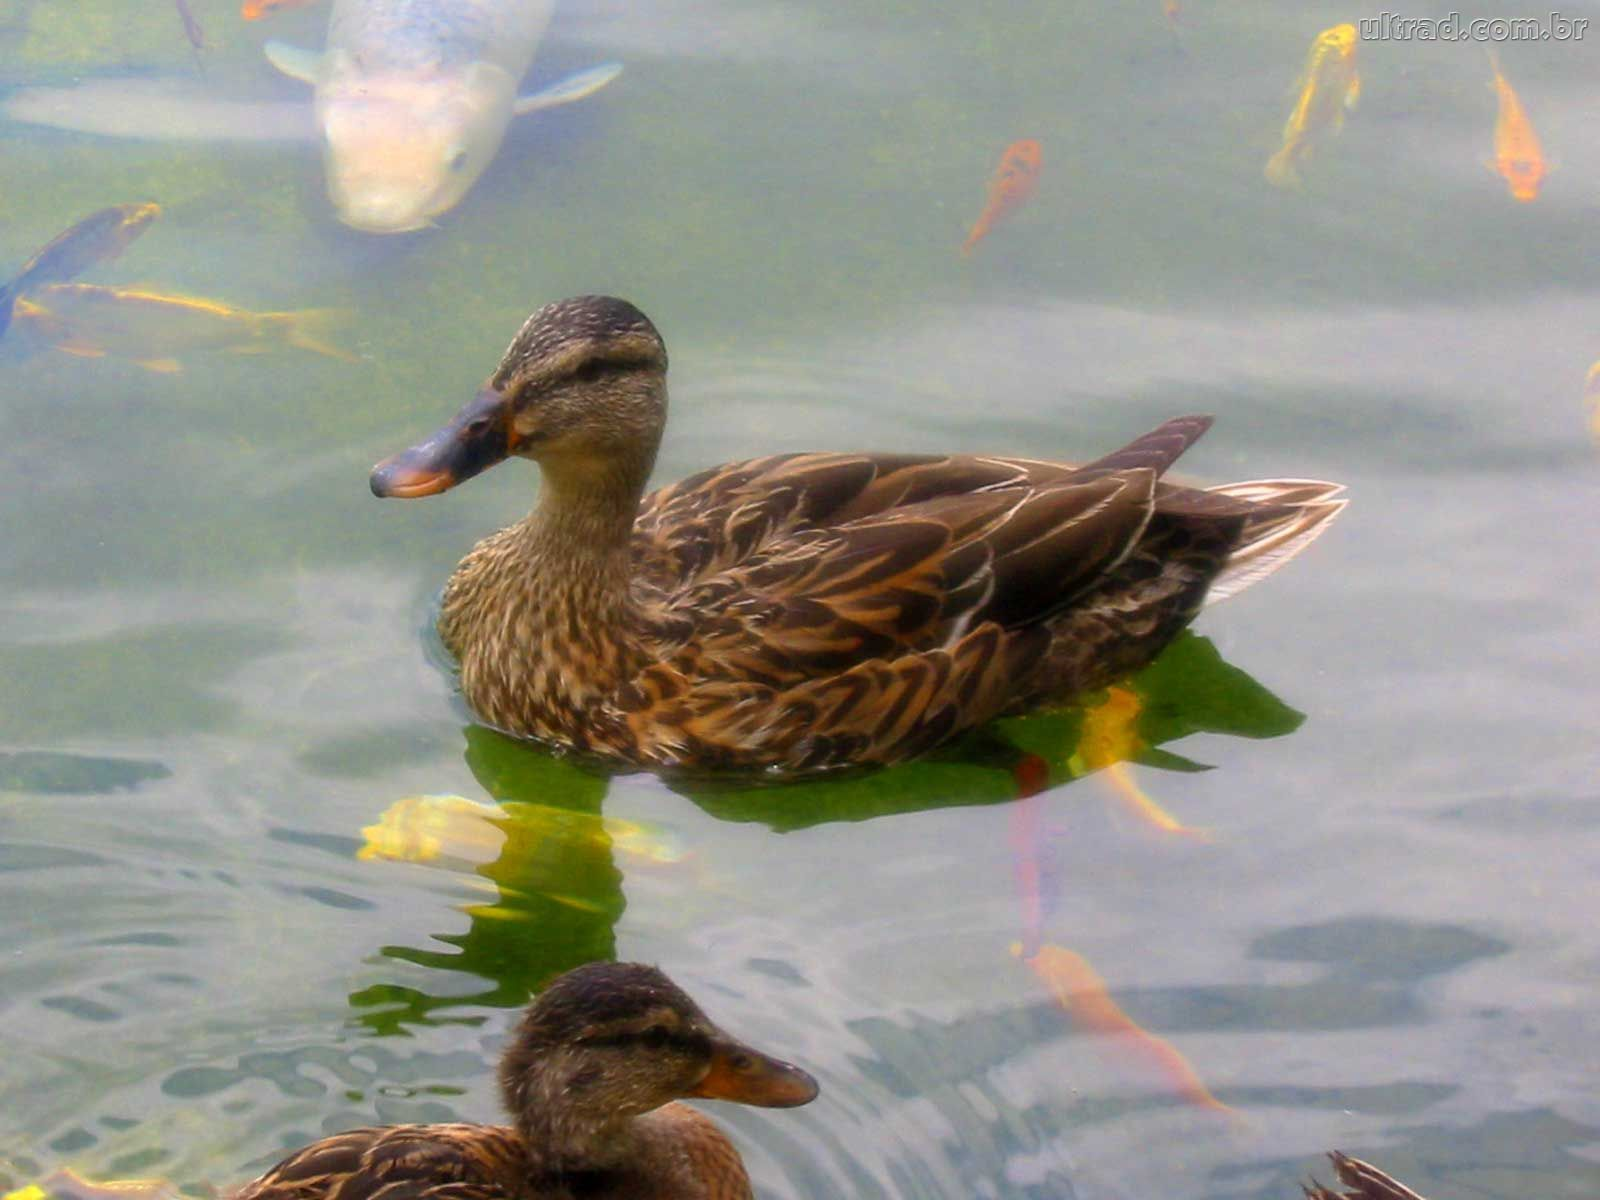
\includegraphics[scale=0.08]{./02-figuras/pato}
  \label{fig:patoA}
\end{center}

Artigos como mais de duas colunas não suportam o ambiente "figure" utilizado neste modelo \LaTeX. Uma alternativa para este problema é a inclusão do pacote:

{\tiny
\begin{verbatim}
    \usepackage{caption}
\end{verbatim}
}

e das seguintes linhas de comando:

{\tiny
\begin{verbatim}
    \begin{center}
      \captionof{figure}{<caption da figura>} 
      \includegraphics[<comandos alternativos>]
      		{<caminho ou nome da figura>}
      \label{<nome da referencia da figura>}
    \end{center}
\end{verbatim}
}



% -----------------------------------------------------------------------------
% Nova subseção
% -----------------------------------------------------------------------------

\subsection{Figura ocupando duas colunas} 		% edite para alterar o título da subseção

O ambiente \verb+figure+ pode ser usado em um artigo quando a figura for centralizada entre as margens do artigo (ocupa um espaço maior que uma coluna). Porém é necessário a introdução do \verb+*+ após o comando \verb+figure+.

\begin{figure*}
	\centering
	\caption{Pato na lagoa. Fator de escala: 20\% da original} 
	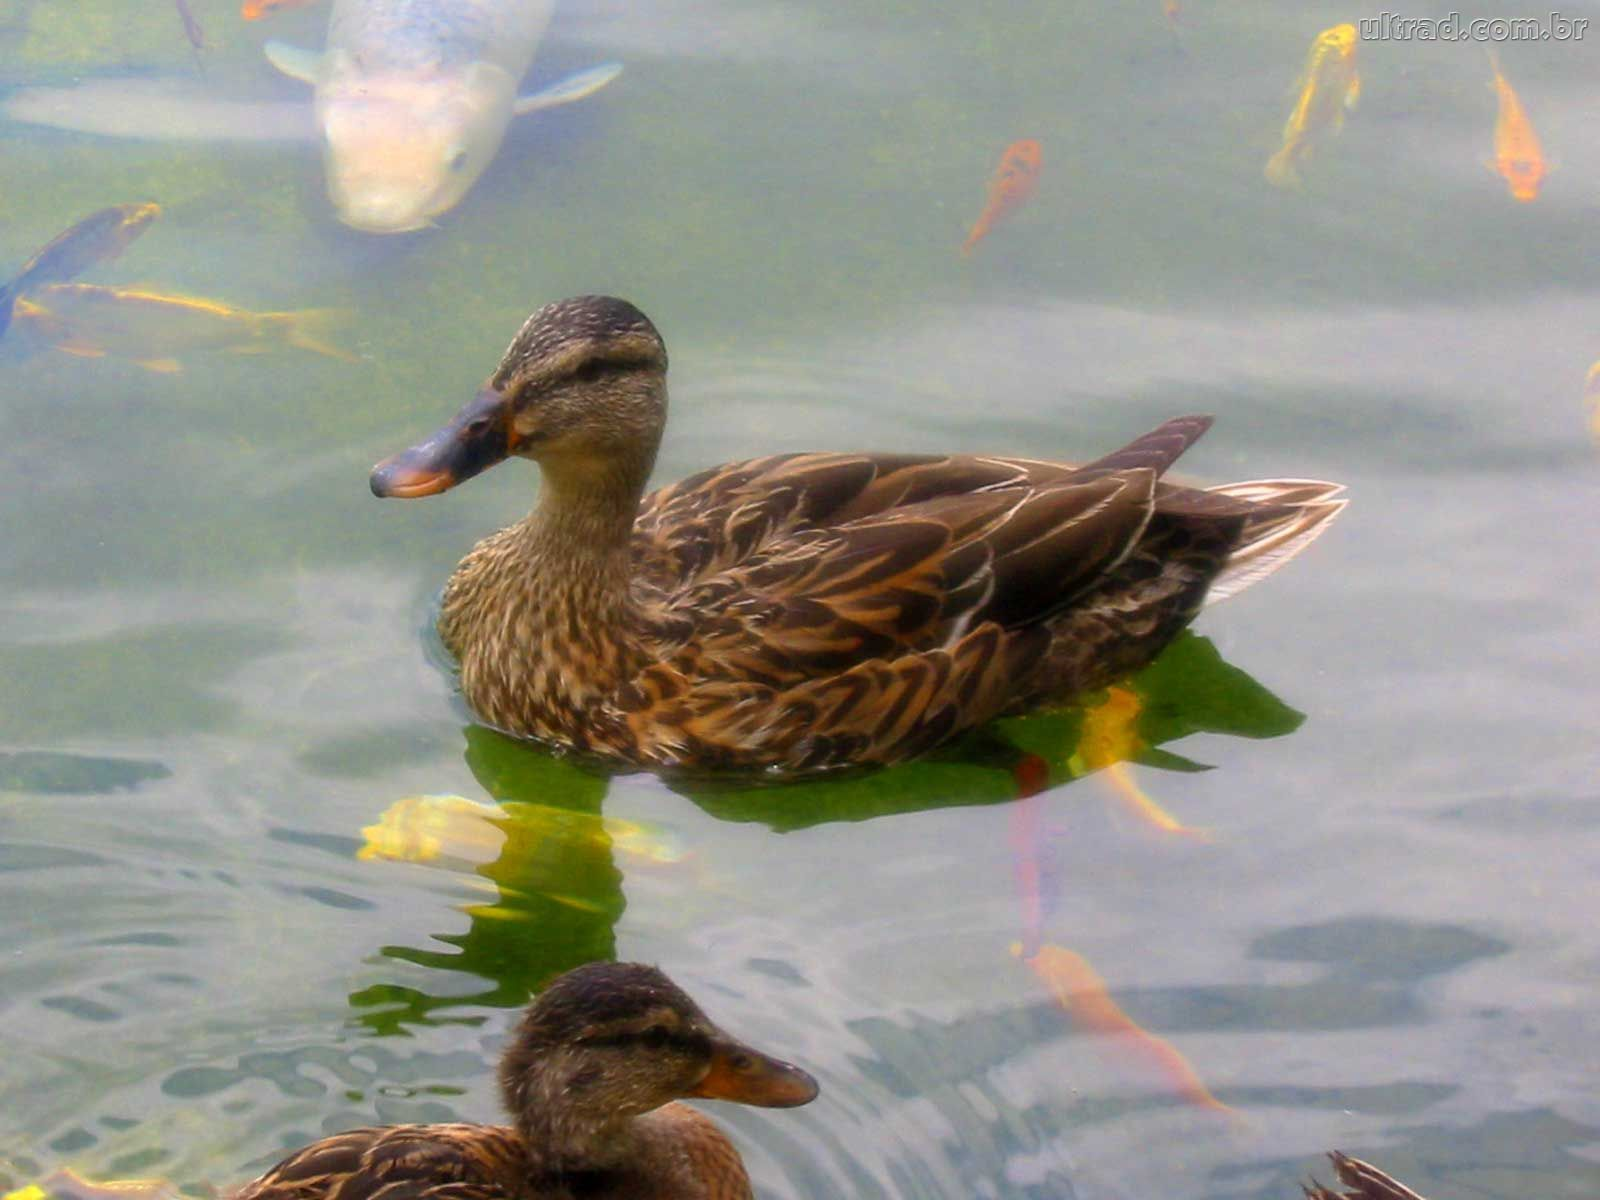
\includegraphics[scale=0.2]{./02-figuras/pato}
	\label{fig:patoB}
\end{figure*}

A \textbf{Figura \ref{fig:patoB}} foi inserida no artigo utilizando o comando \verb+figure*+ para o ambiente de figura.

{\tiny
\begin{verbatim}
   \begin{figure*}
     \centering
     \caption{Pato na lagoa. Fator de escala: 20\% da original} 
     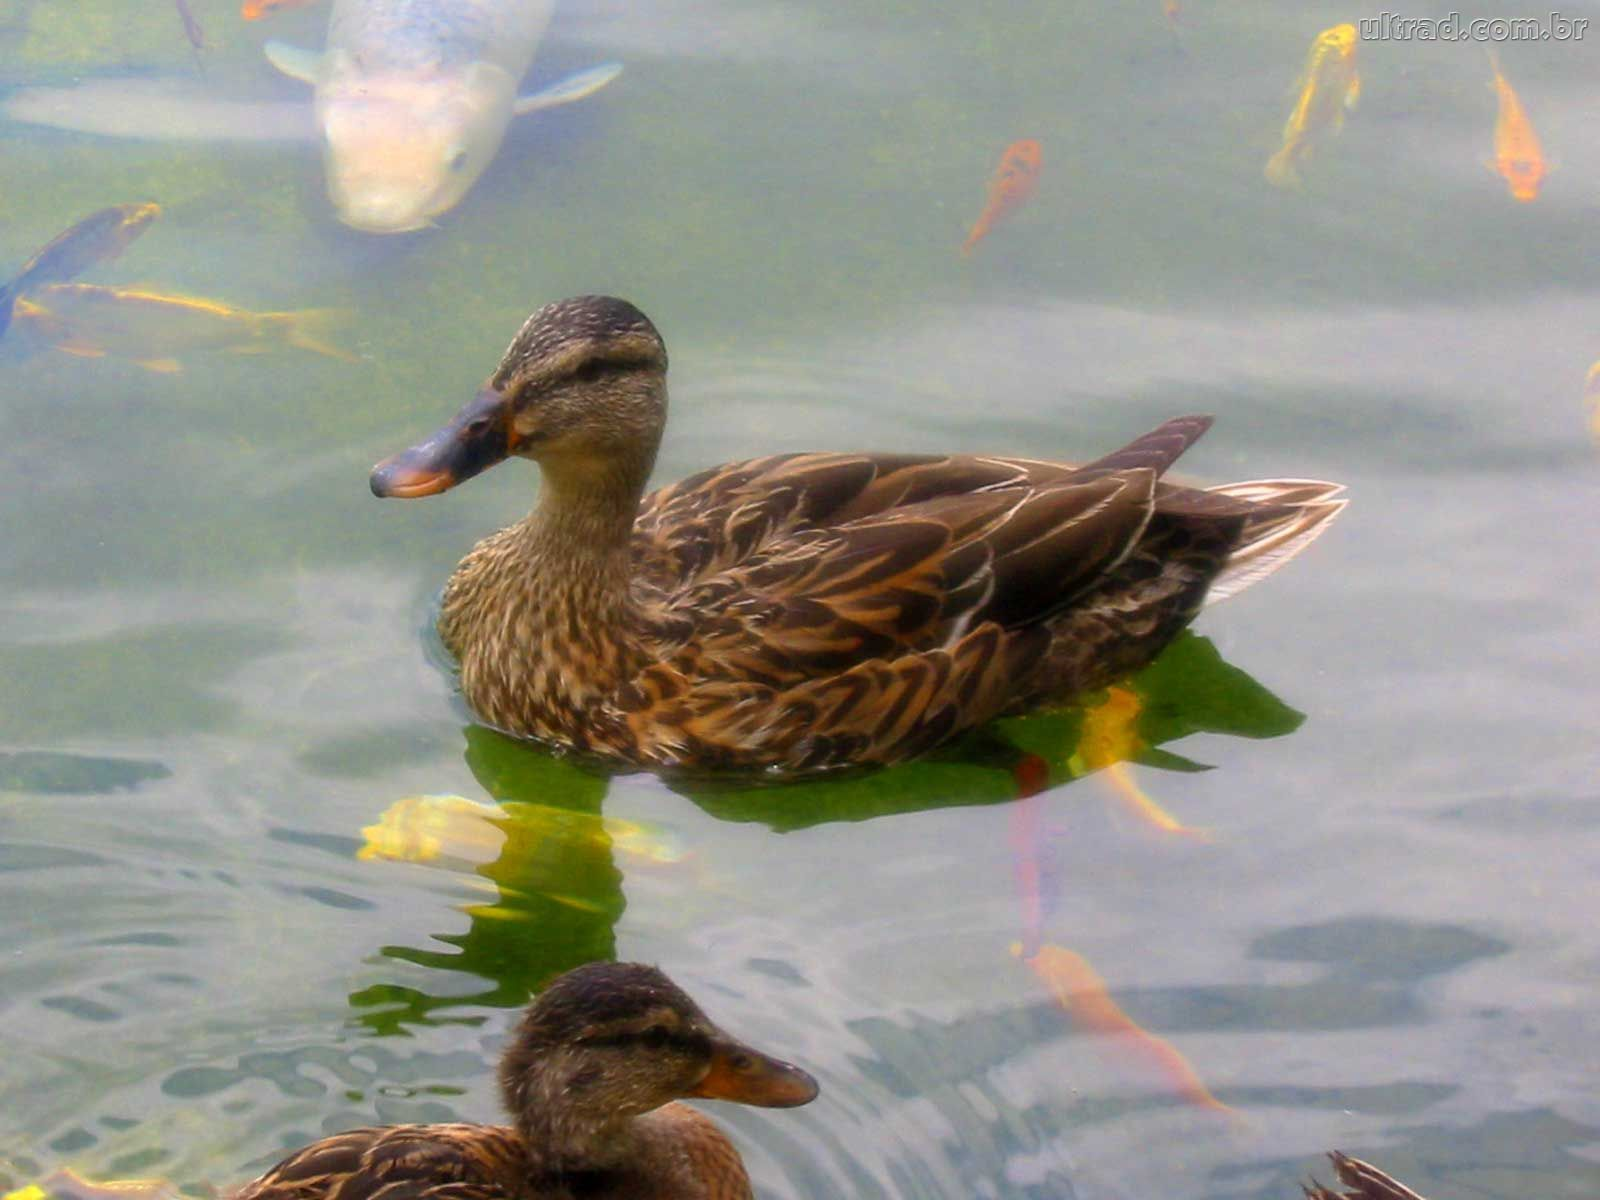
\includegraphics[scale=0.2]{./02-figuras/pato}
     \label{fig:patoB}
   \end{figure*}
\end{verbatim}
}



% -----------------------------------------------------------------------------
% Nova subseção
% -----------------------------------------------------------------------------

\subsection{Tabelas} 		% edite para alterar o título da subseção

O ambiente de tabelas é inserido no texto de modo análogo àquele feito no ambiente de figuras.




% -----------------------------------------------------------------------------
% Nova subseção
% -----------------------------------------------------------------------------

\subsection{Citações de referências} 		% edite para alterar o título da subseção

As referências são inseridas no texto como em qualquer documento em \LaTeX. Quando o nome do autor da referência faz parte do texto que você está escrevendo use o comando  \verb+\citeonline{}+ e quando este não for o caso use o comando \verb+\cite{}+. Veja a diferença entre os dois nas seguintes frases:

\noindent\textbf{(1)} Conforme discute \citeonline{kim1996} o resultado [...].

\noindent\textbf{(2)} Alternativamente a literatura\cite{kim1996} indica que o resultado [...].

Quando se tem mais de uma referência a ser citada em um mesmo certo trecho, há duas possibilidades de referenciá-las:

\noindent\textbf{(1)} colocar todas as referências em um único colchete (\emph{i.e.}, num mesmo comando \verb+\cite+),


\cite{kim1996,Wikibooks2009}

	
\noindent\textbf{(2)} colocar cada referência em seu próprio colchete (\emph{i.e.}, usando vários comandos \verb+\cite+ consecutivos),


\cite{kim1996}\cite{Wikibooks2009}

